\documentclass{article}

\title{Chapter 3 Exercises}
\date{2019-08-01}
\author{Termanteus}

% Used for graph plot
\usepackage{tikz}
\usepackage{pgfplots}
  \pgfplotsset{compat=1.16}

% Section has a dot
\usepackage{titlesec}
  \titlelabel{\thetitle.\quad}

% Dot-filling for ToC's Sections
\usepackage{tocloft}
\renewcommand\cftsecleader{\cftdotfill{\cftdotsep}}

\usepackage{amsmath}
\usepackage{amsfonts}
\usepackage{amssymb}
\usepackage{mathtools}
\DeclarePairedDelimiter{\ceil}{\lceil}{\rceil}
\DeclarePairedDelimiter{\floor}{\lfloor}{\rfloor}

\usepackage{listings}
\usepackage{color}

% Use for table when having overfull hbox
\usepackage{adjustbox}

\usepackage{scrextend}

% For pictures
\usepackage{graphicx}
\usepackage{subcaption}

% For pseudocode
\usepackage[linesnumbered,ruled]{algorithm2e}

\usepackage{filecontents}

\pgfplotstableread[col sep = comma]{prefix_0.csv}\prefixdata
\pgfplotstableread[col sep = comma]{prefix_1.csv}\prefixdataone
\pgfplotstableread[col sep = comma]{prefix_2.csv}\prefixdatatwo
\pgfplotstableread[col sep = comma]{sorted.csv}\sorteddata


\lstset{
  language= Python,
  basicstyle=\small\sffamily,
	numbers=left,
 	numberstyle=\tiny,
	frame=tb,
	tabsize=4,
	columns=fixed,
	showstringspaces=false,
	showtabs=false,
	keepspaces,
	commentstyle=\color{gray},
	keywordstyle=\color{blue}
}

\begin{document}

\maketitle
\pagenumbering{gobble}
\newpage
\pagenumbering{arabic}

\tableofcontents
\newpage



\section{R-3.1}
\paragraph{Statement}
Graph the functions $8n$, $4nlog(n)$, $2n^2$, $n^3$, and $2^n$ using a logarithmic scale
for the x- and y-axes; that is, if the function value $f(n)$ is y, plot this as a
point with x-coordinate at logn and y-coordinate at $log(y)$.
\paragraph{Solution}
Graph:
  \begin{figure}[h]
    \begin{center}
      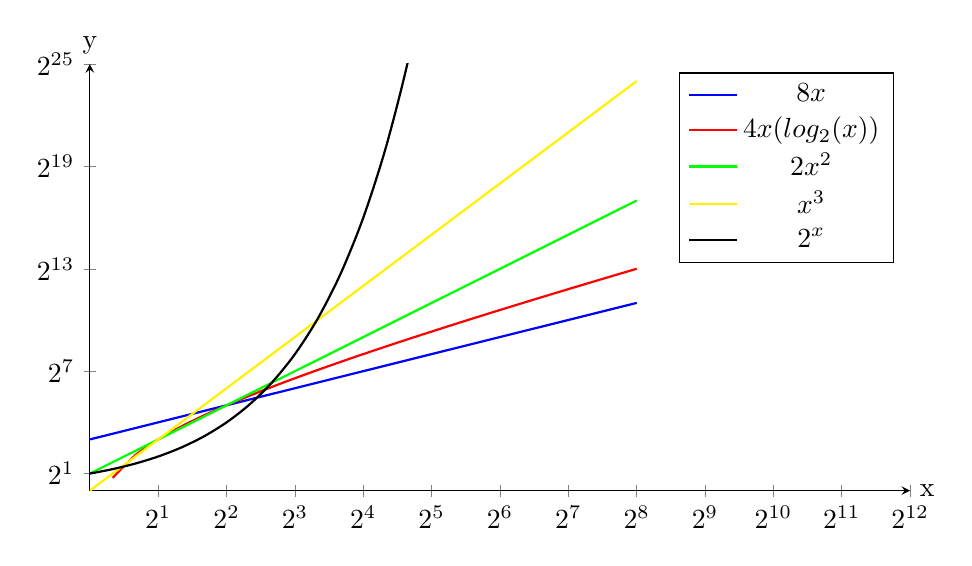
\begin{tikzpicture}
        \begin{axis}[
            xmode=log,
            ymode=log,
            log basis y={2},
            log basis x={2},
            %
            width=12cm,
            height=7cm,
            axis x line=center,
            axis y line=left,   % <-- `center' confuses PGFPlots on a log axis
            xmin=1,
            xmax=4096,
            ymin=1,
            ymax=2^25,
            xlabel={x},
            ylabel={y},
            xlabel style={right},
            ylabel style={
                at={(rel axis cs:0,1)},
                rotate=-90,
                anchor=south,
            },
        ]
            \addplot [smooth,domain=1:256,blue, thick] {8*x};
            \addlegendentry{$8x$}
            \addplot [smooth,domain=1:256,red, thick] {4*x*(ln(x)/ln(2))};
            \addlegendentry{$4x(log_{2}(x))$}            
            \addplot [smooth,domain=1:256,green, thick] {2*x^2};
            \addlegendentry{$2x^2$}
            \addplot [smooth,domain=1:256,yellow, thick] {x^3};
            \addlegendentry{$x^3$}
            \addplot [smooth,domain=1:256,thick] {2^x};
            \addlegendentry{$2^x$}
        \end{axis}
    \end{tikzpicture}
    \end{center}
  \end{figure}

\newpage
\section{R-3.2}
\paragraph{Statement}
The number of operations executed by algorithms A and B is $8nlog(n)$ and
$2n^2$, respectively. Determine $n_{0}$ such that A is better than B for n $>=$ $n_{0}$.
\paragraph{Solution}
Graph:
  \begin{figure}[h]
    \begin{center}
      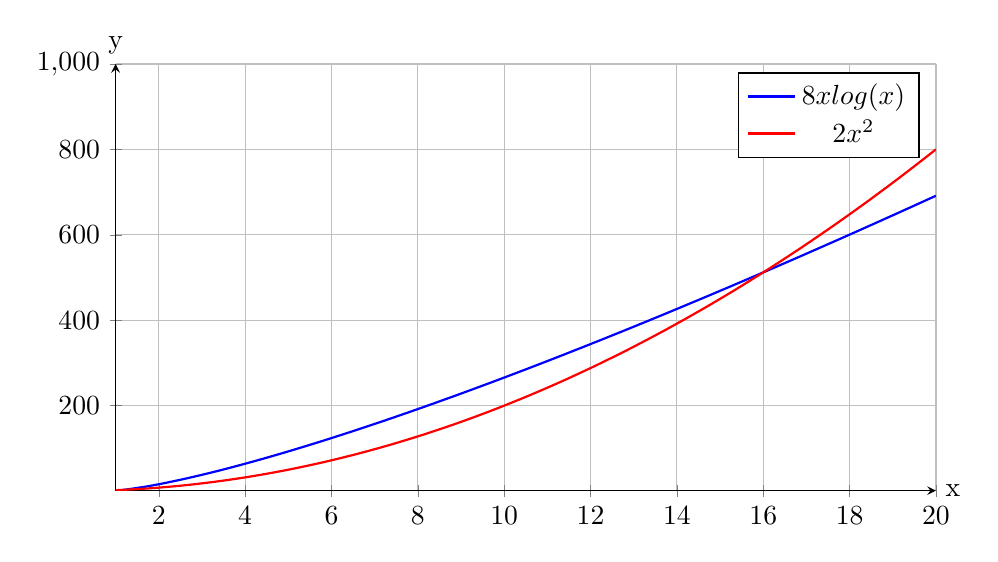
\begin{tikzpicture}
        \begin{axis}[
            width=12cm,
            height=7cm,
            grid=major,
            axis x line=center,
            axis y line=left,   % <-- `center' confuses PGFPlots on a log axis
            xmin=1,
            xmax=20,
            ymin=1,
            ymax=1000,
            xlabel={x},
            ylabel={y},
            xlabel style={right},
            ylabel style={
                at={(rel axis cs:0,1)},
                rotate=-90,
                anchor=south,
            },
        ]
            \addplot [smooth,domain=1:20,blue, thick] {8*x*log2(x)};
            \addlegendentry{$8xlog(x)$}
            \addplot [smooth,domain=1:20,red, thick] {2*x^2};
            \addlegendentry{$2x^2$}            

        \end{axis}
    \end{tikzpicture}
    \caption{As you can see in the graph, at $n>=16$ A is better than B.}
    \end{center}
  \end{figure}

\newpage
\section{R-3.3}
\paragraph{Statement}
The number of operations executed by algorithms A and B is $40n^2$ and
$2n^3$, respectively. Determine $n_{0}$ such that A is better than B for n $>=$ $n_{0}$.
\paragraph{Solution}
Graph:
  \begin{figure}[h]
    \begin{center}
      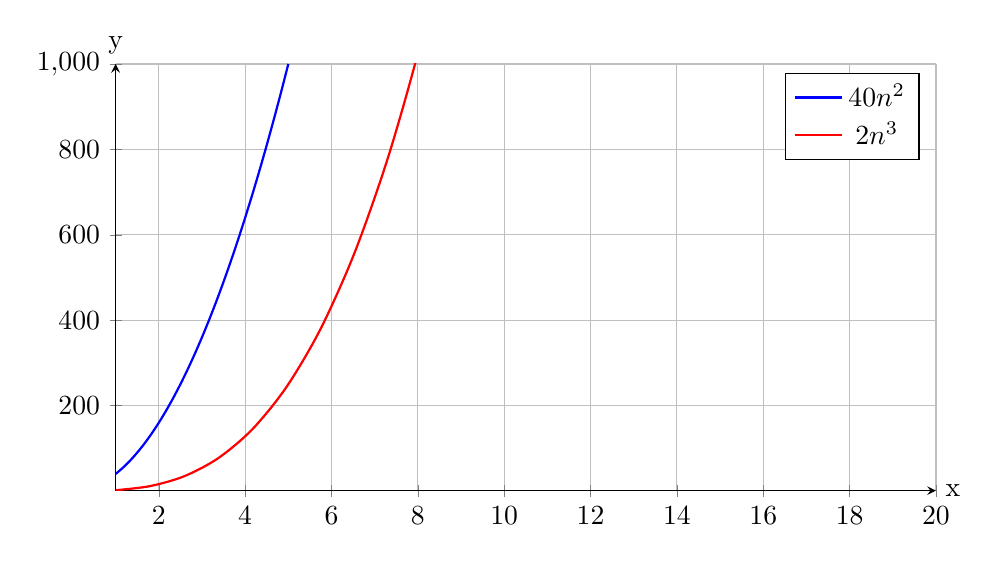
\begin{tikzpicture}
        \begin{axis}[
            width=12cm,
            height=7cm,
            grid=major,
            axis x line=center,
            axis y line=left,   % <-- `center' confuses PGFPlots on a log axis
            xmin=1,
            xmax=20,
            ymin=1,
            ymax=1000,
            xlabel={x},
            ylabel={y},
            xlabel style={right},
            ylabel style={
                at={(rel axis cs:0,1)},
                rotate=-90,
                anchor=south,
            },
        ]
            \addplot [smooth,domain=1:5,blue, thick] {40*x^2};
            \addlegendentry{$40n^2$}
            \addplot [smooth,domain=1:20,red, thick] {2*x^3};
            \addlegendentry{$2n^3$}            

        \end{axis}
    \end{tikzpicture}
    \caption{As you can see in the graph, at $n>=0$ A is better than B.}
    \end{center}
  \end{figure}
\newpage

\section{R-3.4}
\paragraph{Statement}
Give an example of a function that is plotted the same on a log-log scale
as it is on a standard scale.
\paragraph{Solution}
  $f(x)=const$
\section{R-3.5}
\paragraph{Statement}
Explain why the plot of the function nc is a straight line with slope c on a
log-log scale.
\paragraph{Solution}
  We have
  \begin{align*}
      y &= n^c \\
      \Leftrightarrow log(y) &= log(n^c)\\
      \Leftrightarrow log(y) &= clog(n)
  \end{align*}
\paragraph{}
  On a log-log scale graph, we can see $log(n) ~ x$ in a standard graph, so it means that means the function above is a linear function, so the coefficent (c in this situation) is its slope.
\section{R-3.6}
\paragraph{Statement}
What is the sum of all the even numbers from 0 to 2n, for any positive
integer n?
\paragraph{Solution}
  \begin{equation}
    {S} = \frac{n(2+2n)}{2} = {n(n+1)}
  \end{equation}
\section{R-3.7}
\paragraph{Statement}
\setlength{\parindent}{14ex}
Show that the following two statements are equivalent:
\par(a) The running time of algorithm A is always $O(f(n))$.
\par(b) In the worst case, the running time of algorithm A is $O(f(n))$
\setlength{\parindent}{12ex}
\paragraph{Solution}
  As the book said: "Therefore, for the remainder of this book, unless we specify
  otherwise, we will characterize running times in terms of the worst case, as a function of the input size, n, of the algorithm."\par
  So basically the two sentences is the same.
\setlength{\parindent}{0pt}
\section{R-3.8}
\paragraph{Statement}
Order the following functions by asymptotic growth rate.
\paragraph{Solution}
  \begin{align*}
    2^{10} &< 4n < 3n+100log(n) < nlog(n) < ... \\
    ... &< 4nlog(n) + 2n<n^2+10<2^{log(n)}<2^n
  \end{align*}
\section{R-3.9}
\paragraph{Statement}
Show that if $d(n)$ is $O(f(n))$, then $ad(n)$ is $O(f(n))$, for any constant $a > 0$.
\paragraph{Solution}
  Because as the definition has state: $f(n) <= cg(n)$ for $n>=n_{0}$
\section{R-3.10}
\paragraph{Statement}
Show that if $d(n)$ is $O(f(n))$ and $e(n)$ is $O(g(n))$, then the product $d(n)e(n)$
is $O(f(n)g(n))$.
\paragraph{Solution}
  Because as the definition has state: $f(n) <= cg(n)$ for $n>=n_{0}$
  \par So we have 
  \begin{align*}
    d(n)e(n) &<= c_{1}f(n) * c_{2}g(n), \quad n>=n_{0} \\
    \Leftrightarrow d(n)e(n) &<= c_{0}(f(n) * g(n))\\
    \Leftrightarrow d(n)e(n) &<= O(f(n) * g(n))
  \end{align*}

% Set Indent to 12ex for align with Solution
\setlength{\parindent}{12ex}
% Set Indent to 12ex for align with Solution

\section{R-3.11}
\paragraph{Statement}
Show that if $d(n)$ is $O(f(n))$ and $e(n)$ is $O(g(n))$, then the sum of $d(n)+e(n)$
is $O(f(n)+g(n))$.
\paragraph{Solution}
  Because as the definition has state: $f(n) <= cg(n)$ for $n>=n_{0}$
  \par So we have: 
  \begin{align*}
    d(n)e(n) &<= c_{1}f(n) + c_{2}g(n), \quad n>=n_{0}\\
    \Leftrightarrow d(n)e(n) &<= c_{0}(f(n) + g(n))\\
    \Leftrightarrow d(n)e(n) &<= O(f(n) + g(n))
  \end{align*}
\section{R-3.12}
\paragraph{Statement}
Show that if $d(n)$ is $O(f(n))$ and $e(n)$ is $O(g(n))$, then $d(n) - e(n)$
is \textbf{not necessarily} $O(f(n)-g(n))$.
\paragraph{Solution}
  Assume the statement is true:\par
  For example: $d(n) = n^2 = O(n^2)$ and $e(n) = 3n^2 = O(n^2)$\par
  Then: $d(n)-e(n) = O(n^2-n^2) = O(0)$
  $\rightarrow$ \textbf{False}
\section{R-3.13}
\paragraph{Statement}
Show that if $d(n)$ is $O(f(n))$ and $f(n)$ is $O(g(n))$, then $d(n)$
is $O(g(n))$.
\paragraph{Solution}
  Based on the definition, we will have:
  \begin{align*}
    \begin{cases}
    d(n) &<= c_{0}f(n)\\
    f(n) &<= c_{1}g(n)\\
    \end{cases}\\
    \Rightarrow d(n) <= c_{2}g(n)\\
    \Leftrightarrow d(n) = O(g(n))
  \end{align*}
\section{R-3.14}
\paragraph{Statement}
Show that $O(max{f(n),g(n)}) = O(f(n) + g(n))$.
\paragraph{Solution}
  Based on excercise \textbf{3.11} it is proved to be true
\section{R-3.15}
\paragraph{Statement}
Show that $f(n)$ is $O(g(n))$ if and only if $g(n)$ is $\Omega( f (n))$.
\paragraph{Solution}
  Based on \textbf{Big-Omega's definition} and \textbf{Big-O's definition} it is proved to be true.
\newpage
\section{R-3.16}
\paragraph{Statement}
Show that if $p(n)$ is a polynomial in n, then $log(p(n))$ is $O(log(n))$.
\paragraph{Solution}
  \begin{align*}
    p(n) &= \sum_{k=0}^{n} a_{k}x^{k}\\
    \Leftrightarrow log(p(n)) &= log(\sum_{k=0}^{n} a_{k}x^{k})\\
    \Leftrightarrow log(p(n)) &= log(a_{0}x^{0}) + log(a_{1}x^{1}) + ... +log(a_{n}x^{n})\\
    \Leftrightarrow log(p(n)) &= 0*log(a_{0}x) + 1*log(a_{1}x^{1}) + ... + n*log(a_{n}x)\\
    \Leftrightarrow log(p(n)) &= O(log(n))
  \end{align*}
\section{R-3.17}
\paragraph{Statement}
Show that $(x + 1)^5$ is $O(n^5)$.
\paragraph{Solution}
  \begin{align*}
    f(x) &= x^5 + 5*x^4 + 10*x^3 +10*x^2 + 5*x + 1\\
    \Leftrightarrow f(x) &= O(n^50)
  \end{align*}
\section{R-3.18}
  Skip because easy...
\section{R-3.19}
  Skip because easy...
\section{R-3.20}
  Skip because easy...
\section{R-3.21}
  Skip because easy...
\section{R-3.22}
  \paragraph{Statement}
  Show that $\ceil[\bigg] {f(n)}$ is $O( f (n))$, if $f (n)$ is a positive nondecreasing function that is always greater than 1.
  \paragraph{Solution}
    If $f (n)$ is a positive nondecreasing function that is always greater than 1, then $\ceil[\bigg] {f(n)} <= f(n) + 1$ .
\newpage
\lstinputlisting{exercises.py}

\section{R-3.23}
\paragraph{Statement}
Give a big-Oh characterization, in terms of n, of the running time of the example1 function shown in Code Fragment 3.10.
\paragraph{Solution}
  \begin{itemize}
    \item Loop through n items $\rightarrow \ O(n)$.
    \item Each loop do constant $O(1)$ time.
    \item \textbf{Total:} $O(n)$
  \end{itemize}
\section{R-3.24}
\paragraph{Statement}
Give a big-Oh characterization, in terms of n, of the running time of the example2 function shown in Code Fragment 3.10.
\paragraph{Solution}
  \begin{itemize}
    \item Loop through $\ceil{n/2}$ items $\rightarrow \ O(n)$.
    \item Each loop do constant $O(1)$ time.
    \item \textbf{Total:} $O(n)$
  \end{itemize}
\section{R-3.25}
\paragraph{Statement}
Give a big-Oh characterization, in terms of n, of the running time of the example3 function shown in Code Fragment 3.10.
\paragraph{Solution}
  \begin{itemize}
    \item Loop through ($1*2*3*...*(n-1)*n$) items $\rightarrow \ O(n^2)$.
    \item Each loop do constant $O(1)$ time.
    \item \textbf{Total:} $O(n^2)$
  \end{itemize}
\section{R-3.26}
\paragraph{Statement}
Give a big-Oh characterization, in terms of n, of the running time of the example4 function shown in Code Fragment 3.10.
\paragraph{Solution}
  \begin{itemize}
    \item Loop through $n$ items $\rightarrow \ O(n)$.
    \item Each loop do constant $O(1)$ time.
    \item \textbf{Total:} $O(n)$
  \end{itemize}
\section{R-3.27}
\paragraph{Statement}
Give a big-Oh characterization, in terms of n, of the running time of the example5 function shown in Code Fragment 3.10.
\paragraph{Solution}
  \begin{itemize}
    \item Loop through $n*n*(n+1)/2$ items $\rightarrow \ O(n^3)$.
    \item Each loop do constant $O(1)$ time.
    \item \textbf{Total:} $O(n^3)$
  \end{itemize}

\newpage
\section{R-3.28}
\paragraph{Statement}
For each function $f (n)$ and time $t$ in the following table determine the largest size $n$ of a problem P that can be solved in time $t$ if the algorithm for solving P takes $f (n) $ microseconds (one entry is already completed).
\paragraph{Solution}
  We have:\par
  \begin{itemize}
    \item 1 second = $10^6$ microseconds
    \item 1 hour = $3.6*10^9$ microseconds
    \item 1 month = $2.592*10^12$ microseconds
    \item 1 century = $3.1104*10^15$ microseconds
  \end{itemize}

  And we also know that $f(n)$ microseconds will be taken for solving problem P of size n.
  So the maximum problems we can solve for $f(n) = log(n)$ in 1 second is such that:
  \begin{align*}
    log(n) &<= 10^6 \\
    2^{log(n)} &<= 2^{10^6}\\
    n &<= 10^{300000}, \quad 2^{10}\approx 10^3
  \end{align*}
  \begin{table}[h!]
    \begin{center}
        \begin{adjustbox}{width={\textwidth},totalheight={\textheight},keepaspectratio}
        \begin{tabular}{|c|c|c|c|c|}
          \hline
          & \textbf{1 Second} & \textbf{1 Hour}& \textbf{1 Month} & \textbf{1 Century} \\
          \hline
          $logn$ & $\approx 10^{300000}$& $\approx 10^{1080000000}$ & $\approx 10^{7.776*10^{11}}$ & $\approx 10^{9.3312*10^{14}}$        \\
          
          $\sqrt{n}$ & $ 10^{12}$&$\approx 12.96 * 10^{18}$ & $\approx 6.718464 * 10^{24}$ & $\approx 9.67458816 * 10^{30}$           \\
          
          $n$ & $\approx 10^{6}$&$\approx 36*10^{8}$ & $\approx 746496*10^{16}$ & $\approx 995827586973696*10^{16}$       \\
          
          $nlogn$ & 62746& 133378058& 71870856404 & 68654697441062       \\
          
          $n^2$ & 1000& 60000& 1609968 & 56175382         \\
          
          $2^n$ & 19& 31& 41 &51          \\
          \hline
        \end{tabular}
      \end{adjustbox}
    \end{center}
  \end{table}

\section{R-3.29}
  \paragraph{Statement}
  Algorithm A executes an $O(log n)$-time computation for each entry of an n-element sequence. What is its worst-case running time?
  \paragraph{Solution}
  $T=O(nlog(n))$
\newpage
\section{R-3.30}
  \paragraph{Statement}
  Given an n-element sequence S, Algorithm B chooses $logn$ elements in S at random and executes an $O(n)$-time calculation for each. What is the worst-case running time of Algorithm B?
  \paragraph{Solution}
  Assuming picking random index for each element cost constant $O(1)$ time. In such case: $T=O(nlogn)$
\section{R-3.31}
  \paragraph{Statement}
  Given an n-element sequence S of integers, Algorithm C executes an $O(n)$-time computation for each even number in S, and an $O(logn)$-time computation for each odd number in S. What are the best-case and worstcase running times of Algorithm C?
  \paragraph{Solution}
  \textbf{Best case:} All element in S is odd: $T=O(nlogn)$\par
  \textbf{Worst case:} All element in S is even: $T=O(n^2)$
\section{R-3.32}
  \paragraph{Statement}
  Given an n-element sequence S, Algorithm D calls Algorithm E on each element $S[i]$. Algorithm E runs in $O(i)$ time when it is called on element $S[i]$. What is the worst-case running time of Algorithm D?
  \paragraph{Solution}
  $T=O(n)$
\section{R-3.33}
  \paragraph{Statement}
  Al and Bob are arguing about their algorithms. Al claims his $O(nlogn)$-time method is always faster than Bob’s $O(n^2)$-time method. To settle the issue, they perform a set of experiments. To Al’s dismay, they find that if $n < 100$, the $O(n^2)$-time algorithm runs faster, and only when $n >= 100$ is the $O(nlogn)$-time one better. Explain how this is possible
  \paragraph{Solution}
  Based on the definition $f(n) = O(g(n)) \  \text{iff} \  f(n)<=cg(n), \  n>=n_{0} $. So probably for $n<100$ the $O(nlogn)$ is not held.
\newpage
\section{R-3.34}
  \paragraph{Statement}
  There is a well-known city (which will go nameless here) whose inhabitants have the reputation of enjoying a meal only if that meal is the best they have ever experienced in their life. Otherwise, they hate it. Assuming meal quality is distributed uniformly across a person’s life, describe the expected number of times inhabitants of this city are happy with their meals?
  \paragraph{Solution}
  "If the sequence is given to us in random order, the probability that the $j^{th}$ element is the largest of the first j elements is $\frac{1}{j}$ (assuming uniqueness). Hence the expected number of times we see the current biggest (including initialization) is $H_{n} = \sum_{j=1}^{n}\frac{1}{j}$, which is known as the $n^{th}$ \textbf{Harmonic number}."
\section{C-3.35}
  \paragraph{Statement}
  Assuming it is possible to sort n numbers in O(nlogn) time, show that it is possible to solve the three-way set disjointness problem in $O(nlogn)$-time.
  \paragraph{Solution}
  Sort: $O(nlogn)$\par
  Binary Search: $O(logn)$ to search a element in the other two.\par
  T= $O(nlogn)$ 
\section{C-3.36}
  \paragraph{Statement}
  Describe an efficient algorithm for finding the ten largest elements in a sequence of size n. What is the running time of your algorithm?
  \paragraph{Solution}
  Sort: $O(nlogn)$\par
  T= $O(nlogn)$ 
\section{C-3.37}
  \paragraph{Statement}
  Give an example of a positive function $f (n)$ such that $f (n)$ is neither $O(n)$ nor $\Omega(n)$.
  \paragraph{Solution}
  $f(n) = 0*n$
\newpage
\section{C-3.38}
  \paragraph{Statement}
  Show that $\sum_{i=1}^{n}i^2$ is $O(n^3)$
  \paragraph{Solution}
  \begin{align}
    S=\sum_{i=1}^{n}i^2 &= 1^2 + 2^2 + ... + n^2
  \end{align}
  We gonna use Integral Bound for (2) because (2) is a weakly increasing series.
  For 
  \begin{align*}
    I &= \int_{1}^{n}f(x)dx\\
    I &= \int_{1}^{n}x^2dx\\
    I &= \frac{x^3}{3} \Big|_1^n\\
    I &= \frac{n^3}{3} - \frac{1}{3}
  \end{align*}
  We will have:
  \begin{align*}
    I + f(1) <= S &<= I + f(n)\\
    S &<= \frac{n^3}{3} - \frac{1}{3} + n^2\\
    S &= O(n^3)
  \end{align*}

\newpage
\section{C-3.39}
  \setlength{\parindent}{3ex}
  \paragraph{Statement}
  Show that 
  \begin{equation}
    \sum_{i=1}^{n}\frac{i}{2^i} < 2
  \end{equation}
  \paragraph{Solution}
    \begin{align}
      \textbf{Let: }S(x) &= \sum_{i=1}^{n}{i{x}^i}
    \end{align}
    1. We first prove (4) is a convergent series:\par
    \begin{itemize}
      \item {
        \textbf{Radius of convergent: } $(-1,1)$, prove: 
        \begin{align*}
          l &= \lim_{n\rightarrow+\infty}{\sqrt[\leftroot{-2}\uproot{2}n]{|n|}} = 1\\
          r &= \frac{1}{l} = 1 \\
          \intertext{For x = 1:}
          S(1) &= \sum_{i=1}^{n}n \\
          \intertext{$\rightarrow$\textbf{Divergent Series with x = 1.}}
          \intertext{For x = -1:}
          S(1) &= \sum_{i=1}^{n}{n*(-1)^n} \\
          \intertext{$\rightarrow$\textbf{Divergent Series with x = -1.}}
          \intertext{Conclude:}
          x&\in(-1,1)
        \end{align*}
      }
      \newpage
      \item {
        \textbf{Find sum of $S(x)$: }
        \begin{align*}
          \intertext{For $\forall x \in (-1,1)$:}\\
          S(x) &= \sum_{i=1}^{n}{i{x}^i} \\
          S(x) &= x * \sum_{i=1}^{n}{i{x}^{i-1}} \\
          S(x) &= x * \sum_{i=1}^{n}{({x}^{i})'} \\
          S(x) &= x * \Big(\sum_{i=1}^{n}{{x}^{i}}\Big)' \\
          S(x) &= x * \Big(\frac{x}{1-x}\Big)' \\
          S(x) &= \frac{x}{(1-x)^2} \\
        \intertext{Replace $x = \frac{1}{2}, we have:$ }
          S\Big(\frac{1}{2}\Big) &= \frac{\frac{1}{2}}{(1-\frac{1}{2})^2} =2
        \end{align*}
      }
    \end{itemize}
    \newpage
    
\section{C-3.40}
\paragraph{Statement}
Show that $log_{b}{f(n)}$ is $\Theta(logf(n))$ if $b>1$ is a constant.
\paragraph{Solution}
    \begin{align*}
      \intertext{We have basic logarithmic formula: }
      log_{a}b &= \frac{log_{c}b}{log_{c}a}
      \intertext{Similarly we apply to $log_{b}{f(n)}$: }
      log_{b}f(n) &= \frac{log_{2}f(n)}{log_{2}b}\\
      logf(n) &= {log_{b}f(n)}{logb}\\
      \intertext{Apply the Big-Theta definition, we have this statement proved. }
    \end{align*}
\newpage \setlength{\parindent}{12ex}    \section{C-3.41}
  \paragraph{Statement}
  Describe an algorithm for finding both the minimum and maximum of n numbers using fewer than $\frac{3n}{2}$ comparisons. (Hint: First, construct a group of candidate minimums and a group of candidate maximums.)
  \paragraph{Solution}
  Source code:\par
    \lstinputlisting{findMinMax.py}
\newpage \section{C-3.42}
  \paragraph{Statement}
  Bob built a Web site and gave the URL only to his n friends, which he numbered from 1 to n. He told friend number i that he/she can visit the Web site at most i times. Now Bob has a counter, C, keeping track of the total number of visits to the site (but not the identities of who visits). What is the minimum value for C such that Bob can know that one of his friends has visited his/her maximum allowed number of times?
  \paragraph{Solution}
  For everyone (except the first one) visit until they only have one left, the total visited times will be:
  \begin{align*}
    S &= 1 + 2 + ... + n-1\\
    S &= \frac{(n-1)(n-1+1)}{2}\\
    S &= \frac{(n-1)n}{2}
  \intertext{At this time, whoever watch will reach his/her limit, and C will know. So the minimun value for C is:}
    S &= \frac{(n-1)n}{2}+1
  \end{align*}
\section{C-3.43}
  \paragraph{Statement}
  Draw a visual justification of Proposition 3.3  analogous to that of Figure 3.3(b) for the case when n is odd.
  \paragraph{Solution}
  \begin{figure}[b]
    \centering
    \begin{subfigure}[b]{0.75\linewidth}
      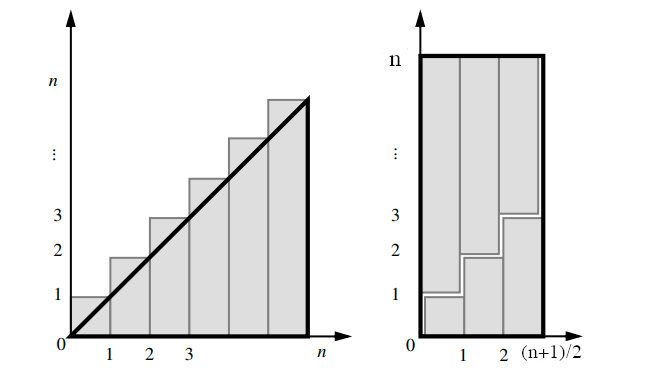
\includegraphics[width=\linewidth]{chart33.png}
      \caption{Proposition 3.3 when n is odd.}
    \end{subfigure}  
  \end{figure}
\section{C-3.44}
  \paragraph{Statement}
  Communication security is extremely important in computer networks, and one way many network protocols achieve security is to encrypt messages. Typical cryptographic schemes for the secure transmission of messages over such networks are based on the fact that no efficient algorithms are known for factoring large integers. Hence, if we can represent a secret message by a large prime number p, we can transmit, over the network, the number $r = p*q$, where $q > p$ is another large prime number that acts as the encryption key. An eavesdropper who obtains the transmitted number r on the network would have to factor r in order to figure out the secret message p. \par Using factoring to figure out a message is very difficult without knowing the encryption key q. To understand why, consider the following naive
factoring algorithm:
  \begin{lstlisting}
    for p in range(2,r):
      if r % p == 0: # if p divides r
    return "The secret message is p!"
  \end{lstlisting}
  \paragraph{Solution}
  a) For a message r has 100 bits, the worst case is when $p=2^{100/2} = 2^{50}$ (because $r = p*q$ and $q>p$). So to decipher message r, this algorithm would have to take $2^{50}$ microseconds $\approx 35$ years  \par
  b) Based on the answer of question a), we have known that the worst scenario is such that $p=2^{m/2}, m=n*8$,with m is the number of bits representing r. So we have to perform $2^{4n}$ divisions to find p. With the complexity of $O(n)$ for each division, the total running time will be $O(n2^{4n})$.
\section{C-3.45}
  \paragraph{Statement}
  A sequence S contains $n-1$ unique integers in the range [0, $n-1$], that is, there is one number from this range that is not in S. Design an $O(n)$-time algorithm for finding that number. You are only allowed to use $O(1)$ additional space besides the sequence S itself.
  \paragraph{Solution}
  Sort, then run from 0 to n-1, if the current number is not equal previous number + 1, then previous number + 1 is the one we need to find.
\newpage \setlength{\parindent}{14ex}\section{C-3.46}
  \paragraph{Statement}
   Al says he can prove that all sheep in a flock are the same color:\par \textit{Base case}: One sheep. It is clearly the same color as itself.\par \textit{Induction step}: A flock of n sheep. Take a sheep, a, out. The remaining $n - 1$ are all the same color by induction. Now put sheep a back in and take out a different sheep, b. By induction, the $n - 1$ sheep (now with a)are all the same color. Therefore, all the sheep in the flock are the same color. What is wrong with Al’s “justification”?
  \paragraph{Solution}
  Al makes an implicit assumption that the set n+1 has at least 3 sheeps. This is not true when n + 1 = 2 sheeps.
\section{C-3.47}
  \paragraph{Statement}
  Let S be a set of n lines in the plane such that no two are parallel and no three meet in the same point. Show, by induction, that the lines in S determine $\Theta(n^2)$ intersection points.
  \paragraph{Solution}
  \par \textit{Base case:} ($n = 0$): 0 lines and 0 intersection
  \par \textit{Induction step:}  ($n > 0$): Assume claim true for n lines. When add one more line to a plane with n lines, since among lines, no two are parallel and no three meet in the same point, it will add $n$ more intersect. So:\par The total intersect with n+1 lines = currentIntersect + $n$, or
  \par The total intersect with n+1 lines = $\Theta(n^2)$ + $O(n)$ = $\Theta(n^2)$
  \par So this holds for n+1 lines while n is true, \textbf{proved}.
\section{C-3.48}
  \paragraph{Statement}
  Consider the following “justification” that the Fibonacci function, $F(n)$ (see Proposition 3.20) is $O(n)$:
  \par \textit{Base case:} ($n <= 2$): $F(1) = 1$ and $F(2) = 2$.
  \par \textit{Induction step:}  ($n > 2$): Assume claim true for $n' < n$. Consider $n$. $F(n) = F(n-2) + F(n-1)$. By induction, $F(n-2)$ is $O(n-2)$ and $F(n-1)$ is $O(n-1)$. Then, $F(n)$ is $O((n-2)+ (n-1))$, by the identity presented in Exercise R-3.11. Therefore, $F(n)$ is $O(n)$.
  \par What is wrong with this “justification”?
  \setlength{\parindent}{12ex}\paragraph{Solution}
  This "justification" is equivalent to proving a number is $O(1)$. So whenever you plug in a value of n to the function $F(n)$, you turn it into a constant, not a function anymore.
  
\section{C-3.49}
  \paragraph{Statement}
  Consider the Fibonacci function, $F(n)$ (see Proposition 3.20). Show by induction that $F(n)$ is $\Omega\Bigg(\Big(\frac{3}{2}\Big)^n\Bigg)$.
  \paragraph{Solution}
  \par \textit{Base case:} ($n = 0$): 0 lines and 0 intersection
  \par \textit{Induction step:}  ($n > 0$): Assume claim true for n = k, which means:
  \begin{align*}
    &F(k) <= c * \Big(\frac{3}{2}\Big)^n, \quad n>=n_{0}, c \in \text{R} \\
    &F(k+1) = F(k) + F(k-1)\\
    &F(k+1) = \Omega\Bigg(\Big(\frac{3}{2}\Big)^n\Bigg) + \Omega\Bigg(\Big(\frac{3}{2}\Big)^n\Bigg) \\
    &F(k+1) = \Omega\Bigg(\Big(\frac{3}{2}\Big)^n\Bigg)
    \intertext{This mean that k+1 still holds if k is true, \textbf{proved}.}
  \end{align*}
\newpage \section{C-3.50}
  \paragraph{Statement}
  Let $p(x)$ be a polynomial of degree n, that is, $p(x) = \sum_{i=0}^{n}a_{i}x^{i}$.
  \par (a) Describe a simple $O(n^2)$-time algorithm for computing $p(x)$.
  \par (b) Describe an $O(nlogn)$-time algorithm for computing $p(x)$, based upon a more efficient calculation of $x^i$.
  \par (c) Now consider a rewriting of $p(x)$ as
  \begin{equation*}
    p(x) = a_{0} + x\Big(a_{2} + x\big(a_{3}+...+x(a_{n-1}+xa_{n})...)\big)\Big)
  \end{equation*}\\
  which is known as \textbf{Horner’s method}. Using the big-Oh notation, characterize the number of arithmetic operations this method executes
  \paragraph{Solution}
  For-loop conventions: For $i=0$ to n, the loop will stop when $i=n-1$. reverse(i=0 to n) will corresponding to n-1,n-2,...0 
  \begin{algorithm}[h!]
    \SetKwInOut{Input}{Input}
    \SetKwInOut{Output}{Output}

    \underline{function evaluatePolynomial} $(coefficents,x)$\;
    \Input{Array of corresponding coefficent for each $x_{i}$,x }
    \Output{Sum of the polynomial}
    $sum \longleftarrow 0$\;
    $size \longleftarrow len(coefficents)$\;
    \For{$i=0$ to size}{
      $power \leftarrow 1$\;
      \For{$j=1$ to i+1}{
        $power \leftarrow power * x$;
      }
      $sum \leftarrow coefficents[i] * power$
    }
    \KwRet{$sum$}\;
    \caption{A simple $O(n^2)$-time algorithm for computing $p(x)$}
  \end{algorithm}
  \newpage
  \begin{algorithm}[t!]
    \SetKwInOut{Input}{Input}
    \SetKwInOut{Output}{Output}

    \underline{function evaluatePolynomial} $(coefficents,x)$\;
    \Input{Array of corresponding coefficent for each $x_{i}$,x }
    \Output{Sum of the polynomial}
    $sum \longleftarrow 0$\;
    $size \longleftarrow len(coefficents)$\;
    \For{$i=0$ to size}{
      \If {i is odd}{
        $power \leftarrow x$\;
      }
      \Else{
        $power \leftarrow 1$\;
      }
      \For {$j=0$ to $\ceil{log(i)}$}{
        $power \leftarrow power * x^2$;
      }
      $sum \leftarrow coefficents[i] * power$
    }
    \KwRet{$sum$}\;
    \caption{An improved $O(nlogn)$-time algorithm for computing $p(x)$, based upon a more efficient calculation of $x^i$.}
  \end{algorithm}
  
  \begin{algorithm}[h!]
    \SetKwInOut{Input}{Input}
    \SetKwInOut{Output}{Output}

    \underline{function evaluatePolynomial} $(coefficents,x)$\;
    \Input{Array of corresponding coefficent for each $x_{i}$, x }
    \Output{Sum of the polynomial}
    $sum \longleftarrow 0$\;
    \For{i=reverse(0 to size)}{
      $sum \leftarrow coefficents[i]+ x*sum$
    }
    \KwRet{$sum$}\;
    \caption{\textbf{Horner’s method}}
  \end{algorithm}
  \noindent \textbf{Running time}: O(n), also O(n) multiplication.

\newpage \section{C-3.51}
\paragraph{Statement}
Show that the summation $\sum_{i=1}^{n}log(i)$ is $O(nlogn)$.
\paragraph{Solution}
Let P(n): $\sum_{i=1}^{n}log(i) <= nlogn$\par
\textit{Base case:} $P(1) = 0 <= 0$. \textbf{True}\par
\textit{Inductive step:} Assume P(n) true, prove P(n+1) true:
\begin{align*}
  \sum_{i=1}^{n+1}log(i)&= \sum_{i=1}^{n}log(i) + log(n+1)\\
  \sum_{i=1}^{n+1}log(i)&<= nlog(n) + log(n+1), \quad\text{with}\\
  nlog(n) + log(n+1)&<= nlog(n+1) + log(n+1)\\
  \sum_{i=1}^{n+1}log(i)&<= (n+1)log(n+1)
  \intertext{So P(n+1) holds when P(n) is true. \textbf{Proved}.}
  \intertext{Based on the definition of Big-Oh, we have $\sum_{i=1}^{n}log(i)$ is $O(nlogn)$}
\end{align*}
\section{C-3.52}
\paragraph{Statement}
Show that the summation $\sum_{i=1}^{n}log(i)$ is $\Omega(nlogn)$.
\paragraph{Solution}
We can see that $\sum_{i=1}^{n}log(i) >= \sum_{i=n/2}^{n}log(i)$ 
\par Also:
  \begin{align*}
    \sum_{i=n/2}^{n}log(i) &>= \frac{n}{2}*log(\frac{n}{2})\\
    \sum_{i=n/2}^{n}log(i) &>= \frac{n}{2}*(log(n)-log(2))\\
    \sum_{i=n/2}^{n}log(i) &= \Omega(nlogn)
  \end{align*}
\newpage \section{C-3.53}
\paragraph{Statement}
An evil king has n bottles of wine, and a spy has just poisoned one of them. Unfortunately, they do not know which one it is. The poison is very deadly; just one drop diluted even a billion to one will still kill. Even so, it takes a full month for the poison to take effect. Design a scheme for determining exactly which one of the wine bottles was poisoned in just one month’s time while expending $O(logn)$ taste testers.
\paragraph{Solution}
To represent number n in bits we must use $k = \floor {log(n)} + 1$ bits
\par Then we will use k people to test n bottles, mark each person/bottle with number from $1\rightarrow n$. Then the rule to determine who will try which bottle is this: \textbf{With the number of that person converted to binary number, who has the value 1 at the $i^{th}$ bit will try the $i^{th}$ bottle. If he/her dies alone, then the bottle of has  $(2^{\textbf{that man's number}-1})$ is poison, if more than one dies, $(\textbf{OR of their number})^{th}$ bottle has poison.}
\par For example: 8 bottles, 4 people:
  \begin{align*}
    0001\\
    0010\\
    0011\\
    0100\\
    0101\\
    0110\\
    0111\\
    1000\\
    \intertext{Person 1: bottle 1,3,5,7; Person 2: 2,3,6,7; Person 3: 4,5,6,7; Person 4: 8}
    \intertext{If P1 dies: 1; If P2 dies: 2; If P3 dies: 4;If P4 dies: 8}
    \intertext{If P1,P2 dies: 3, and so on...}
  \end{align*}
\section{C-3.54}
\paragraph{Statement}
A sequence S contains n integers taken from the interval $[0,4n]$, with repetitions allowed. Describe an efficient algorithm for determining an integer value k that occurs the most often in S. What is the running time of your algorithm?
\paragraph{Solution}
  Use a map, $T = O(n)$
\section{P-3.55-3.56}
\paragraph{Statement}
Perform an experimental analysis of the three algorithms prefix average1, prefix average2, and prefix average3, from Section 3.3.3. Visualize their running times as a function of the input size with a log-log chart.\paragraph{Solution}
\begin{figure}[h]
  \begin{center}
    \begin{tikzpicture}
        \begin{axis}[
            xmode=log,
            ymode=log,
            log basis y={2},
            log basis x={2},
            %
            width=12cm,
            height=7cm,
            axis x line=center,
            axis y line=left,   % <-- `center' confuses PGFPlots on a log axis
            xmin=2,
            xmax=2^30,
            ymin=1,
            ymax=1024,
            xlabel={Size},
            ylabel={Time},
            xlabel style={right},
            ylabel style={
                at={(rel axis cs:0,1)},
                rotate=-90,
                anchor=south,
            },
        ]
          \addplot table[x index = {0}, y index = {1}]{\prefixdata};
          \addlegendentry{$prefix_0$}
          \addplot table[x index = {0}, y index = {1}]{\prefixdataone};
           \addlegendentry{$prefix_1$}
          \addplot table[x index = {0}, y index = {1}]{\prefixdatatwo};
           \addlegendentry{$prefix_2$}
        \end{axis}
      \end{tikzpicture}
    \end{center}
  \end{figure}
  
\newpage \section{P-3.57}
\paragraph{Statement}
Perform experimental analysis to test the hypothesis that Python sorted method runs in $O(nlogn$)-time on average. 
\begin{figure}[h]
  \begin{center}
    \begin{tikzpicture}
        \begin{axis}[
            xmode=log,
            log basis x={2},
            %
            width=12cm,
            height=7cm,
            axis x line=center,
            axis y line=left,
            xmin=2,
            xmax=2^30,
            ymin=0,
            ymax=100,
            % ytick={0,0.1,0.2,...,1},
            xlabel={Size},
            ylabel={Time},
            xlabel style={right},
            ylabel style={
                at={(rel axis cs:0,1)},
                rotate=-90,
                anchor=south,
            },
        ]
          \addplot table[x index = {0}, y index = {1}]{\sorteddata};
        \end{axis}
      \end{tikzpicture}
    \end{center}
  \end{figure}
\newpage \section{C-3.58}
\paragraph{Statement}
 For each of the three algorithms, unique1, unique2, which solve the element uniqueness problem, perform an experimental analysis to determine the largest value of n such that the given algorithm runs in one minute or less.
\paragraph{Solution}
    \textbf{unique1}: 60.0125 for $n = 2^14 + 2^10 + 2^9$
    \textbf{unique2}: 59.96 for $n = 2^25 + 2^21$
\end{document}